This section describes the deliberation process of the agent based in the practical reasoning theory called BDI (Belief-Desires-Intention) model. This model approach to a reasoning of the agent with limited resources and capabilities, opening the process to the idea of uncertainly which in cases with highly dynamic conditions it have demonstrated to be successful. Understand the BDI model imply understand how its three key features works.

The beliefs represent knowledge or fact about its environment. In this case, the knowledge was encapsulate by the belief manager, described in previous section. This knowledge can vary on time and in wide range of manners.

The desires are goals that the agent wants to achieve. In a practical point of view the desires represent the ideal state of the world for an agent.

The intentions represent the commitment with the agents some of its desires, it means that the agent not only pursuit the accomplishment of its desires but also plan how to act in concordance to them. Depend on how strong the commitment is, the intention lead the agent to take action.

\subsection{Goals life-cycle}

The deliberation process is summarized in a simultaneous evaluation of agent's goals, in which the goals acquire different states.

\begin{figure}
	\centering
	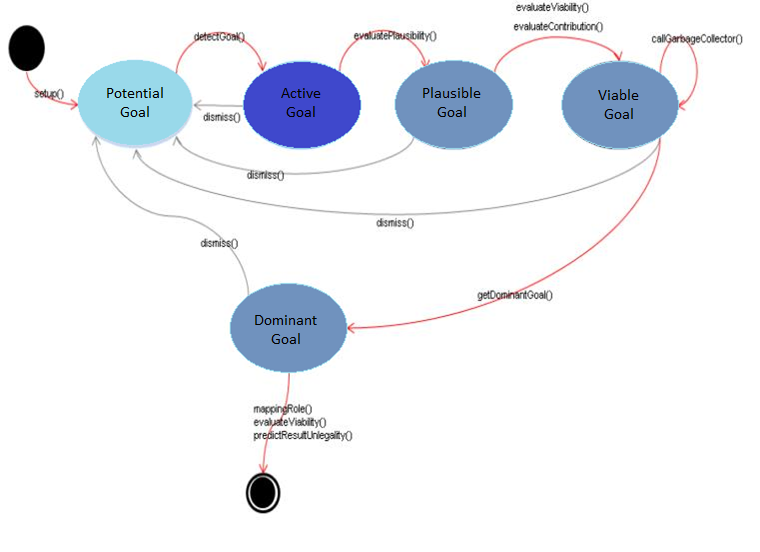
\includegraphics[width=0.5\textwidth]{Images/GoalManagement.png} 
	\caption{GoalManagement. This figure show the goal states in his life-cycle.}
	\label{fig:GoalManager}
\end{figure}

The goals the agent knows are those  delegated by the script and those that are attached to the robotic behavior, like recharge batteries or preserve its own integrity. These goals receive the name of potential goals. 

When a potential goal satisfies its preconditions the goal becomes an active goal. At this point, the agent check if are exists the abilities and resources needed to complete the goal. If not, the goal remains as a potential goal. If there is enough tools and resources the goal becomes a viable goal. 

Finally to the decide what of the viable goals becomes an intention, they compete in two aspects. First, the goals compete by priority, the agent with maximum priority wins. If there is more than one in the maximum priority the goals compete with their contribution values and probability of success (which is an estimated).

\subsubsection{Expropriation and Perseverance}

When an goal becomes an intention the agent deal with indecision problems in real-time. The agent handle when an intention is expropriated by another or when it is maintain.

Expropriation occurs naturally in BDI deliberative process. This happens because the current intention still compete as a potential goal. Then, if some other goal becomes an intention automatically take the place of the current intention. On contrast, if the "winner" goal is the current intention, it maintains as an intention.

However to guarantee some commitment of the agent with his current intention the agent gives a boost in goal's contribution value. In this way, the agent show preference for his current intention when have to decide between several goals. However, despite of the boost, clearly the expropriation is still possible, when the contribution level  is significantly less in compare to another goal or the 


\subsection{Cooperation Manager}

The cooperation manager is on charge of communication with other robo-actor agents. For this purpose is proposed a specialized channel of communication when the messages are FIPA compliant. Two steps are considered in the process of cooperation, which is included directly influence the BDI model. 

Firstly, a simple step, only through implicit synchronization guided by the script, in which participants are clearly described when a cooperative action is needed.

This first step allow to both agents perceive a specific desire as cooperative, and be ready for negotiation. As it is guided for the script the script has an explicit definition of a cooperative action, with this information the belief system can create the delegated goals marking those who needs cooperation.

\todo[inline]{Could be included in the script the possibility of timing information for the action}

The second stage is much more complex and requires a communication protocol that ends with the commitment of parts involved in the cooperation. 

\subsubsection{Protocol for robo-actors}

When an agent set a cooperative delegated goal as a desire immediately search for the ideal partners for achieve it. Then the first message is send  as a petition to the group of ideal partners. At this point every partner cannot reply to the message for lack of interest in the cooperative action or ignorance about the action. at the other hand in the positive case, the agent reply affirmative to the source of petition.

The agent source of the petition acquires the responsibility of determine when the cooperative desire is possible or impossible based on the numbers of agents that have been response willing to cooperate. When the desire becomes possible the agent send a synchronization signal that also works as a commitment message, putting the cooperative desire as an intention

This both steps described above, allows effective coordination within the BDI model. 

\todo[inline]{Example}